\documentclass[review]{elsarticle}
\usepackage{comment}
\usepackage{url}
%
\usepackage[breaklinks]{hyperref}
\usepackage{breakurl}


\usepackage[ruled]{algorithm2e}

\usepackage{blkarray}

%\usepackage{lineno}
%\modulolinenumbers[5]

\journal{Optics Communications}

%%%%%%%%%%%%%%%%%%%%%%%
%% Elsevier bibliography styles
%%%%%%%%%%%%%%%%%%%%%%%
%% To change the style, put a % in front of the second line of the current style and
%% remove the % from the second line of the style you would like to use.
%%%%%%%%%%%%%%%%%%%%%%%

%% Numbered
%\bibliographystyle{model1-num-names}

%% Numbered without titles
%\bibliographystyle{model1a-num-names}

%% Harvard
%\bibliographystyle{model2-names.bst}\biboptions{authoryear}

%% Vancouver numbered
%\usepackage{numcompress}\bibliographystyle{model3-num-names}

%% Vancouver name/year
%\usepackage{numcompress}\bibliographystyle{model4-names}\biboptions{authoryear}

%% APA style
%\bibliographystyle{model5-names}\biboptions{authoryear}

%% AMA style
%\usepackage{numcompress}\bibliographystyle{model6-num-names}

%% `Elsevier LaTeX' style
\bibliographystyle{elsarticle-num}
%%%%%%%%%%%%%%%%%%%%%%%
\usepackage[]{graphicx}

%%%%%%%%%%%%%%%%%%%%%%%%%%%%%%%%%%%%%%%%%%%%%%%%%%%%%%%%%%%%%%%%%%%%%%%%%%%%%%%%%%

\usepackage[svgnames]{xcolor} % Enabling colors by their 'svgnames'

\usepackage{amsmath}
\usepackage{amsfonts}
\usepackage{amssymb}
%%%%%%%%%%%%%%%%%%%%%%%%%%%%%%%%%%%%%%%%%%%%%%%%%%%%%%%%%%%%%%%%%%%%%%%%%%%%%%%%%%

 
\begin{document} 

\begin{frontmatter}

\title{Relation Between the Mass-Spring System and the Dynamic Speckle}
%\tnotetext[mytitlenote]{Fully documented templates are available in the 
%elsarticle package on \href{http://www.ctan.org/tex-archive/macros/latex/contrib/elsarticle}{CTAN}.}



% Group authors per affiliation:
\author{-------- ------- ------}
\author{-------- ------- ------}



% \author{Fernando Pujaico Rivera\fnref{myfootnote2}}
% \author{Roberto Alves Braga Jr.\fnref{myfootnote1}}
% \address{University Federal of Lavras, Lavras, Brazil}
% \fntext[myfootnote2]{201518201@posgrad.ufla.br}
% \fntext[myfootnote1]{robertobraga@deg.ufla.br }


\begin{abstract}
In this article will be studied the relation between the mass-spring system and the dynamic speckle.
\end{abstract}

\begin{keyword}
Biospeckle laser \sep 
Biospeckle signal\sep 
Dynamic speckle \sep  
\end{keyword}

\end{frontmatter}

\linenumbers

%%%%%%%%%%%%%%%%%%%%%%%%%%%%%%%%%%%%%%%%%%%%%%%%%%%%%%%%%%%%%%%%%%%%%%%%%%%%%%%%%%%%%%%%%
%%%%%%%%%%%%%%%%%%%%%%%%%%%%%%%%%%%%%%%%%%%%%%%%%%%%%%%%%%%%%%%%%%%%%%%%%%%%%%%%%%%%%%%%%
\section{Introduction}
The biospeckle laser analysis has presented as a versatile tool in the analysis of
biological activity. 

%%%%%%%%%%%%%%%%%%%%%%%%%%%%%%%%%%%%%%%%%%%%%%%%%%%%%%%%%%%%%%%%%%%%%%%%%%%%%%%%%%%%%%%%%
%%%%%%%%%%%%%%%%%%%%%%%%%%%%%%%%%%%%%%%%%%%%%%%%%%%%%%%%%%%%%%%%%%%%%%%%%%%%%%%%%%%%%%%%%
\section{System description}
The Fig. \ref{fig:system2}.a) represents the signal $z$ with samples $z(n)$, 
obtained  in a pixel of a dynamic speckle analysis,
where $E[z]$ indicates the mean value of $z$. 
\begin{figure}[ht!]
\centering
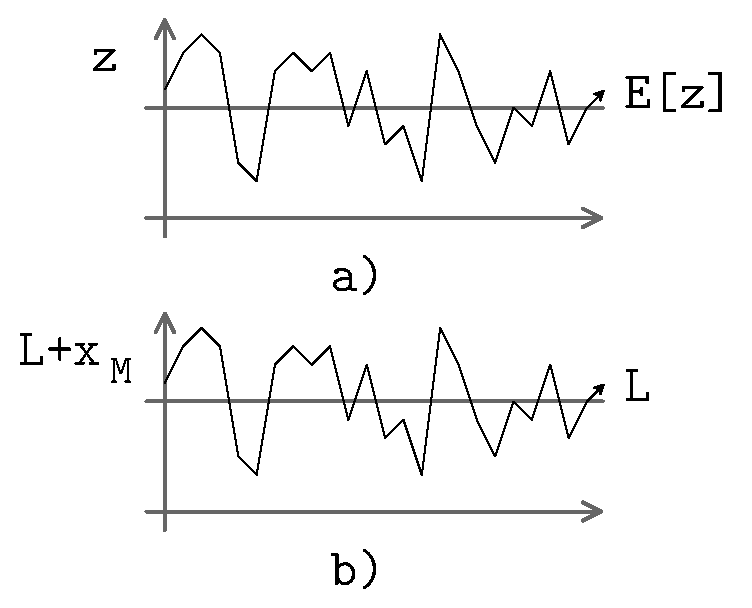
\includegraphics[width=0.55\columnwidth]{images/system-mass-spring-2.eps}
\caption{Data acquisition system setup of the coffee seed.  }
\label{fig:system2}
\end{figure}
Be other side the 
Fig. \ref{fig:system2}.b) represents the signal $x_M$ with samples $x_{M}(n)$, 
obtained  in a mass-spring system of $M$ elements, where each mass
is separated of another by a distance of $L/M$, like can be seen in the
Fig. \ref{fig:system}.
\begin{figure}[ht!]
\centering
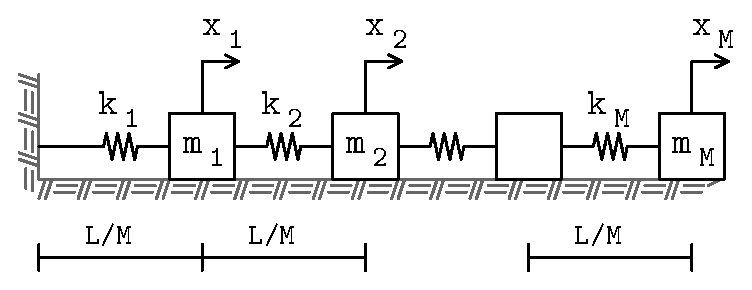
\includegraphics[width=0.95\columnwidth]{images/system-mass-spring.eps}
\caption{Data acquisition system setup of the coffee seed.  }
\label{fig:system}
\end{figure}
Thus, in this system the mass are denoted as $m_i$, the springs as $k_i$ and the
displacements of each mass by $x_i$, for all $1 \leq  i\leq M$.

The objective of this work it is to solve the next inverse problem: Known $y(n)$, 
\begin{equation}\label{eq:yn}
 y(n)=z(n)-E[z]
\end{equation} 
and assuming
$M$ elements with $m_i=m=1/L$; what values of $k_i$ generate a signal $x_M$ that minimize $E$, 
where
\begin{equation}\label{eq:inverseproblem}
 E=\frac{1}{2}\sum_{n} (y(n)-x_M(n))^2
\end{equation} 

%%%%%%%%%%%%%%%%%%%%%%%%%%%%%%%%%%%%%%%%%%%%%%%%%%%%%%%%%%%%%%%%%%%%%%%%%%%%%%%%%%%%%%%%%
%%%%%%%%%%%%%%%%%%%%%%%%%%%%%%%%%%%%%%%%%%%%%%%%%%%%%%%%%%%%%%%%%%%%%%%%%%%%%%%%%%%%%%%%%
\section{Mass-spring system}
Assuming a mass spring system like seen in the Fig. \ref{fig:system} with $m_i=m$
we can to get the system of Eq. (\ref{eq:massspring1}).

\begin{equation}\label{eq:massspring1}
 m \mathbb{\ddot{X}} = -\mathbf{P} \mathbb{X},
\end{equation}
where
\begin{equation}\label{eq:X}
 \mathbb{X} = \left( 
 \begin{matrix}
 x_1\\
 x_2\\ 
 x_3\\ 
 \vdots \\
 x_{N-1}\\
 x_N\\
 \end{matrix}
\right)
\end{equation}
and 
\begin{equation}\label{eq:P}
 \mathbf{P}(\mathbf{K}) \equiv \mathbf{P} = \left( 
 \begin{matrix}
 k_1+k_2 & -k_2    & 0       &  \hdots & 0           & 0  \\
 -k_2    & k_2+k_3 & -k_3    &  \hdots & 0           & 0  \\
 0       &    -k_3 & k_3+k_4 &  \hdots & 0           & 0  \\
 \vdots  & \vdots  & \vdots  &  \ddots & \vdots      & \vdots \\
 0       & 0       & 0       &  \hdots & x_{N-1}+x_N & -x_N  \\
 0       & 0       & 0       &  \hdots & -x_N        & x_N  \\
 \end{matrix}
\right),
\end{equation}
so that $\mathbf{P}$ is a function of $\mathbf{K}=( k_1~ k_2~ k_3~ \hdots ~ k_{M-1}~ k_M)^{T}$.


%%%%%%%%%%%%%%%%%%%%%%%%%%%%%%%%%%%%%%%%%%%%%%%%%%%%%%%%%%%%%%%%%%%%%%%%%%%%%%%%%%%%%%%%%
\subsection{Exact solution}
Knowing the system shown in the Eq. (\ref{eq:massspring1}), we can solve It
using the Eq. (\ref{eq:Xt}),
\begin{equation}\label{eq:Xt}
 \mathbb{X}(t)= \mathbf{V}\left(\mathbf{D}_1 cos(\mathbf{w}t) + \mathbf{D}_2 sin(\mathbf{w}t) \right),
\end{equation}
or Eq. (\ref{eq:Xtalt})
\begin{equation}\label{eq:Xtalt}
 \mathbb{X}(t)= \mathbf{V}\left( cos(\mathbf{W}t)\mathbf{d}_1 +  sin(\mathbf{W}t)\mathbf{d}_2 \right),
\end{equation}
where, $\mathbf{V}=\left( e_1,e_2,\dots ,e_M\right)$ and 
$\mathbf{w}=\left( \sqrt{\lambda_1},\sqrt{\lambda_2},\dots ,\sqrt{\lambda_M}\right)^{T}$ 
are a matrix and a column 
vector conform using the eigenvectors $e_i$ and eigenvalues $\lambda_i$ of
$\mathbf{P}/m$, being $\mathbf{W}$ a diagonal matrix conform with the elements of vector $\mathbf{w}$.
By other side, $\mathbf{D}_1$ and $\mathbf{D}_2$ are two any constant diagonal matrices
conform by the elements of column vectors $\mathbf{d}_1$ and $\mathbf{d}_2$ respectively.
Thus, we now that $\dot{\mathbb{X}}(t)$ and $\ddot{\mathbb{X}}(t)$ are defined by the Eqs. (\ref{eq:dXt_dt})
and (\ref{eq:d2Xt_dt2}) respectively.
\begin{equation}\label{eq:dXt_dt}
 \dot{\mathbb{X}}(t)= \mathbf{V}\left(-\mathbf{D}_1 \mathbf{W} sin(\mathbf{w}t) + \mathbf{D}_2 \mathbf{W} cos(\mathbf{w}t) \right),
\end{equation}
\begin{equation}\label{eq:d2Xt_dt2}
 \ddot{\mathbb{X}}(t)= -\mathbf{V}\left(\mathbf{D}_1 \mathbf{W}^2 cos(\mathbf{w}t) + \mathbf{D}_2 \mathbf{W}^2 sin(\mathbf{w}t) \right),
\end{equation}
thus, It is fulfill that $\mathbf{W}^2=(V D_1)^{-1}(P/m)(V D_1)=(V D_2)^{-1}(P/m)( D_2)$.

\subsubsection{Constant values from two points}
Now, to get the constant values in the column vectors $\mathbf{d}_1$ and $\mathbf{d}_2$, we can
use the Eq. (\ref{eq:d1d2})
\begin{equation}\label{eq:d1d2}
  \left( 
 \begin{matrix}
\mathbf{V}cos(\mathbf{W}t_1) & \mathbf{V}sin(\mathbf{W}t_1)\\
\mathbf{V}cos(\mathbf{W}t_2) & \mathbf{V}sin(\mathbf{W}t_2)\\
 \end{matrix}
 \right)^{-1}
 \left( 
 \begin{matrix}
\mathbb{X}(t_1) \\
\mathbb{X}(t_2)
 \end{matrix}
 \right)=
  \left( 
 \begin{matrix}
\mathbf{d}_1 \\
\mathbf{d}_2
 \end{matrix}
 \right)
\end{equation}

\subsubsection{Constant values from position and velocity of a point}
Now, to get the constant values in the column vectors $\mathbf{d}_1$ and $\mathbf{d}_2$, we can
use the Eq. (\ref{eq:d1d22})
\begin{equation}\label{eq:d1d22}
  \left( 
 \begin{matrix}
\mathbf{V}cos(\mathbf{W}t_1) & \mathbf{V}sin(\mathbf{W}t_1)\\
-\mathbf{V}\mathbf{W}sin(\mathbf{W}t_1) & \mathbf{V}\mathbf{W}cos(\mathbf{W}t_1)\\
 \end{matrix}
 \right)^{-1}
 \left( 
 \begin{matrix}
\mathbb{X}(t_1) \\
\dot{\mathbb{X}}(t_1)
 \end{matrix}
 \right)=
  \left( 
 \begin{matrix}
\mathbf{d}_1 \\
\mathbf{d}_2
 \end{matrix}
 \right)
\end{equation}

%%%%%%%%%%%%%%%%%%%%%%%%%%%%%%%%%%%%%%%%%%%%%%%%%%%%%%%%%%%%%%%%%%%%%%%%%%%%%%%%%%%%%%%%%
\subsection{Finite differences: Knowing two consecutive samples}
\label{subsec:findiff1}
Applying finite differences we known that $\mathbb{X} \equiv \mathbb{X}(n)$ and
$\mathbb{\ddot{X}} \equiv$ $( \mathbb{X}(n+1)$ $-2\mathbb{X}(n)$ $+\mathbb{X}(n-1) ) /{\tau^2}$,
so that the Eq. (\ref{eq:massspring1}) can be rewrite as
\begin{equation}\label{eq:massspring2}
 \mathbb{X}(n) = \left(2 \mathbf{I} -\mathbf{P}\frac{\tau^2}{m}\right) \mathbb{X}(n-1)-\mathbb{X}(n-2),
\end{equation}
now deriving $\mathbb{X}(n)$ by the vector $\mathbf{K}=( k_1~ k_2~ k_3~ \hdots ~ k_{M-1}~ k_M)$,
so that $\mathbb{J}(n) \equiv \frac{\partial \mathbb{X}(n)}{\partial \mathbf{K}}$,
we get the Eq.  (\ref{eq:massspring3})
\begin{equation}\label{eq:massspring3}
 \mathbb{J}(n) = 
 -\frac{\tau^2}{m}\bigcup_{i}{ \left[ \frac{ \partial \mathbf{P} }{\partial k_{i}}  \mathbb{X}(n-1)\right] }
 +\left(2 \mathbf{I} -\mathbf{P}\frac{\tau^2}{m}\right) \mathbb{J}(n-1)
 -\mathbb{J}(n-2),
\end{equation}
where 
\begin{equation}\label{eq:dPdki}
 \frac{ \partial \mathbf{P}}{\partial k_{i}} = 
 \begin{blockarray}{ccccccc}
 ~       & ~       & i-th    & ~       & ~           & ~  & ~\\
 \begin{block}{(cccccc)c}
 0       & 0       & 0       &  \hdots & 0           & 0  & ~\\
 0       & 1       & -1      &  \hdots & 0           & 0  & ~\\
 0       & -1      & 1       &  \hdots & 0           & 0  & i-th\\
 \vdots  & \vdots  & \vdots  &  \ddots & \vdots      & \vdots & ~\\
 0       & 0       & 0       &  \hdots & 0           & 0  & ~\\
 0       & 0       & 0       &  \hdots & 0           & 0  & ~\\
\end{block}
\end{blockarray}
,
\end{equation}


%%%%%%%%%%%%%%%%%%%%%%%%%%%%%%%%%%%%%%%%%%%%%%%%%%%%%%%%%%%%%%%%%%%%%%%%%%%%%%%%%%%%%%%%%
\subsection{Finite differences: Knowing one sample and velocity}
In this case, It is necessary define $\mathbb{\dot{X}} = \mathbb{V}$, so that
the Eq. (\ref{eq:massspring1}) can be rewrite as
\begin{equation}\label{eq:massspringm2}
\left(
\begin{matrix}
 \mathbb{\dot{X}}\\
 \mathbb{\dot{V}}\\
\end{matrix}\right)=
\left(
\begin{matrix}
 \mathbf{0}    & \mathbb{I}_{M \times M} \\
 -\mathbf{P}/m & \mathbf{0} \\
\end{matrix}\right)
\left(
\begin{matrix}
 \mathbb{X}\\
 \mathbb{V}\\
\end{matrix}\right),
\end{equation}
so that we got
\begin{equation}\label{eq:massspringm2a}
 \mathbb{\dot{U}}=A\mathbb{U},
\end{equation}
where $\mathbb{U}= \left( \mathbb{X} ; \mathbb{V} \right)$ and
$A=\left( \mathbf{0} , \mathbb{I}_{M \times M} ; -\mathbf{P}/m , \mathbf{0} \right)$.

Applying finite differences we known that $\mathbb{U} \equiv \mathbb{U}(n)$ and
$\mathbb{\dot{U}} \equiv$ $( \mathbb{U}(n)$ $-\mathbb{U}(n-1)$ $ ) /{\tau_2}$, 
so that the Eq. (\ref{eq:massspringm2a}) can be rewrite as
\begin{equation}\label{eq:massspring2m2}
 \mathbb{U}(n) = \left( \mathbf{I} -\mathbf{A}\tau_2 \right)^{-1} \mathbb{U}(n-1),
\end{equation}
\textcolor{red}{Problems  with finite differences: To got a good aproximation it 
is necessary to choose $\tau_2 \gg \tau$ (where $\tau$ is the value used in the section \ref{subsec:findiff1}). Experimentaly was see that $\tau_2 \geq \tau^2$.}

Now deriving $\mathbb{U}(n)$ by the vector $\mathbf{K}=( k_1~ k_2~ k_3~ \hdots ~ k_{M-1}~ k_M)$,
so that $\mathbb{Q}(n) \equiv \frac{\partial \mathbb{U}(n)}{\partial \mathbf{K}}$,
we get the Eq.  (\ref{eq:massspring3m2})
\begin{equation}\label{eq:massspring3m2}
 \mathbb{Q}(n) = 
  \tau_2 \left( \mathbf{I} -\mathbf{A}\tau_2 \right)^{-1} \bigcup_{i}{ \left[ \frac{ \partial \mathbf{A} }{\partial k_{i}}  \mathbb{U}(n)\right] },
 +\left( \mathbf{I} -\mathbf{A}\tau_2 \right)^{-1} \mathbb{Q}(n-1),
\end{equation}
where 
\begin{equation}\label{eq:dPdkim2}
 \frac{ \partial \mathbf{A} }{\partial k_{i}} = 
\left(
\begin{matrix}
 \mathbf{0}    & \mathbf{0}_{M \times M} \\
 -\frac{1}{m}\frac{ \partial\mathbf{P}}{\partial k_{i}} & \mathbf{0} \\
\end{matrix}\right)
,

\end{equation}
%%%%%%%%%%%%%%%%%%%%%%%%%%%%%%%%%%%%%%%%%%%%%%%%%%%%%%%%%%%%%%%%%%%%%%%%%%%%%%%%%%%%%%%%%
%%%%%%%%%%%%%%%%%%%%%%%%%%%%%%%%%%%%%%%%%%%%%%%%%%%%%%%%%%%%%%%%%%%%%%%%%%%%%%%%%%%%%%%%%
\section{Minimization problem}
The minimization problem seen in the Eq. (\ref{eq:inverseproblem}) can be rewrite as
\begin{equation}\label{eq:minimization1}
 E(\mathbf{K})=\frac{1}{2}\sum_{n} \left( y(n)-\mathbf{B}^{T}\mathbb{X}(n,\mathbf{K}) \right)^2
\end{equation}
where $\mathbf{B}=( 0~ 0~ 0~ \hdots ~ 0~ 1)^{T}$, $y(n)$ are known values and 
$\mathbb{X}(n)$ that is a function of $\mathbf{K}=( k_1~ k_2~ k_3~ \hdots ~ k_{M-1}~ k_M)^{T}$.

Now, knowing that a minimum of $E(\mathbf{K})$ in $\mathbf{K}$ is found when 
$\frac{\partial E(\mathbf{K})}{\partial k_i}=0$ for all integer $1 \leq i \leq M$; we calculate the
Eq. (\ref{eq:minimization1d}).
\begin{equation}\label{eq:minimization1d}
 \frac{\partial E(\mathbf{K})}{\partial k_i}=\sum_{n}{\left( \mathbf{B}^{T}\frac{\partial \mathbb{X}(n,\mathbf{K})}{\partial k_i}\right)^{T} \left( \mathbf{B}^{T}\mathbb{X}(n,\mathbf{K}) -y(n)  \right) },
\end{equation}

Now reordering the Eq. 
(\ref{eq:minimization1d}) using a vectorial differentiation by $\mathbf{K}$, we get the 
Eq. (\ref{eq:minimization2}).
\begin{equation}\label{eq:minimization2}
 \frac{\partial E(\mathbf{K})}{\partial \mathbf{K}}=\sum_{n}{ \left( \mathbf{B}^{T}\mathbb{J}(n,\mathbf{K})\right)^{T} \left(\mathbf{B}^{T}\mathbb{X}(n,\mathbf{K}) -y(n) \right) },
\end{equation}

where $\mathbb{J}(n)=\frac{\partial \mathbb{X}(n)}{\partial \mathbf{K}}$.

%%%%%%%%%%%%%%%%%%%%%%%%%%%%%%%%%%%%%%%%%%%%%%%%%%%%%%%%%%%%%%%%%%%%%%%%%%%%%%%%%%%%%%%%%
\subsection{Landweber iterative method}
The Landweber iteration method propose that 
the minimization of a nonlinear function $E(\mathbf{K})$ can be found using
the gradient descent method, so that 

\begin{equation}\label{eq:Landweber1}
\mathbf{K}_{j}\leftarrow \mathbf{K}_{j-1} - \alpha \frac{\partial E(\mathbf{K}_{j-1})}{\partial \mathbf{K}}
\end{equation}
where $0 < \alpha < 2/||\frac{\partial E(\mathbf{K})}{\partial \mathbf{K}}||^2$ and
$\|\cdot \|$ is the spectral norm. Thus, following the Landweber iteration method
and using the Eq. (\ref{eq:minimization2}) in
our minimization problem, It can be solved using the Eq. (\ref{eq:Landweber2}).
\begin{equation}\label{eq:Landweber2}
\mathbf{K}_{j}\leftarrow \mathbf{K}_{j-1} 
- \alpha \sum_{n}{ \left( \mathbf{B}^{T}\mathbb{J}(n,\mathbf{K}_{j-1})\right)^{T} \left(\mathbf{B}^{T}\mathbb{X}(n,\mathbf{K}_{j-1}) -y(n) \right) }
\end{equation}
%%%%%%%%%%%%%%%%%%%%%%%%%%%%%%%%%%%%%%%%%%%%%%%%%%%%%%%%%%%%%%%%%%%%%%%%%%%%%%%%%%%%%%%%%
\subsection{Tikhonov iterative method}

If we assume that the problem of to get $\mathbf{K}$ will be solved iteratively, 
we can  rewrite the Eq. (\ref{eq:minimization2}) as if was evaluated by $\mathbb{X}_{j}(n)$
and $\mathbb{J}_{j-1}(n)$, as in the Eq. (\ref{eq:miniterative}).
\begin{equation}\label{eq:miniterative}
\sum_{n}{\left\{ \left( \mathbf{B}^{T}\mathbb{J}_{j-1}(n)\right)^{T} \left(\mathbf{B}^{T}\mathbb{X}_{j}(n) - y(n)  \right) \right \}}=\mathbf{0}.
\end{equation}
Where $\mathbb{J}_{j-1}(n)=\mathbb{J}(n,\mathbf{K}_{j-1})$ and
$\mathbb{X}_{j}(n)=\mathbb{X}(n,\mathbf{K}_{j-1})$.

Knowing by the Taylor theorem that 
$\mathbb{X}_{j}(n) \approx \mathbb{X}_{j-1}(n) + \mathbb{J}_{j-1}(n)\left( \mathbf{K}_{j} - \mathbf{K}_{j-1}\right) $

\begin{equation}\label{eq:miniterative2}
\mathbf{K}_{j} = \mathbf{K}_{j-1} +
\left(\sum_{n}{ \left( \mathbf{B}^{T}\mathbb{J}_{j-1}(n)\right)^{T}\left(  \mathbf{B}^{T}\mathbb{J}_{j-1}(n) \right) }\right)^{-1} 
\sum_{n}{ \left( \mathbf{B}^{T}\mathbb{J}_{j-1}(n)\right)^{T} \left(y(n) - \mathbf{B}^{T}\mathbb{X}_{j-1}(n) \right) }.
\end{equation}

joint with the Eqs. (\ref{eq:massspring2}) and (\ref{eq:massspring3}) we got:
\begin{equation}\label{eq:massspring2b}
 \mathbb{X}(n,\mathbf{K}) = \left(2 \mathbf{I} -\mathbf{P(\mathbf{K})}\frac{\tau^2}{m}\right) \mathbb{X}(n-1,\mathbf{K})-\mathbb{X}(n-2,\mathbf{K}),
\end{equation}

\begin{equation}\label{eq:massspring3b}
 \mathbb{J}(n,\mathbf{K}) = 
 -\frac{\tau_2^2}{m}\bigcup_{i}{ \left[ \frac{ \partial\left(\mathbf{P}\right)}{\partial k_{i}}  \mathbb{X}(n-1,\mathbf{K})\right] }
 +\left(2 \mathbf{I} -\mathbf{P(\mathbf{K})}\frac{\tau_2^2}{m}\right) \mathbb{J}(n-1,\mathbf{K})
 -\mathbb{J}(n-2,\mathbf{K}),
\end{equation}
%%%%%%%%%%%%%%%%%%%%%%%%%%%%%%%%%%%%%%%%%%%%%%%%%%%%%%%%%%%%%%%%%%%%%%%%%%%%%%%%%%%%%%%%%
%%%%%%%%%%%%%%%%%%%%%%%%%%%%%%%%%%%%%%%%%%%%%%%%%%%%%%%%%%%%%%%%%%%%%%%%%%%%%%%%%%%%%%%%%
\section{Numerical results} 
\label{sec:numerical}
oioio


%%%%%%%%%%%%%%%%%%%%%%%%%%%%%%%%%%%%%%%%%%%%%%%%%%%%%%%%%%%%%%%%%%%%%%%%%%%%%%%%%%%%%%%%%
%%%%%%%%%%%%%%%%%%%%%%%%%%%%%%%%%%%%%%%%%%%%%%%%%%%%%%%%%%%%%%%%%%%%%%%%%%%%%%%%%%%%%%%%%
\section{Conclusion} 

In this work were presented

\section{Acknowledgment}
We wish to acknowledge the partial financial support for this study provided by the $CAPES$ 
scholarship
$PNPD$ Program, $FAPEMIG$ and $CNPQ$.

%----------------------------------------------------------------------------------------
%	REFERENCE LIST
%----------------------------------------------------------------------------------------
\section{Bibliography}
\bibliography{report}   %>>>> bibliography data in report.bib
\bibliographystyle{spiebib}   %>>>> makes bibtex use spiebib.bst


%----------------------------------------------------------------------------------------

\end{document} 
